% This file was converted from HTML to LaTeX with
% gnuhtml2latex program
% (c) Tomasz Wegrzanowski <maniek@beer.com> 1999
% (c) Gunnar Wolf <gwolf@gwolf.org> 2005-2010
% Version : 0.4.
\section*{Drawing}
Diese Seite dokumentiert die Funktionen der beiden Klassen Drawing und DrawingAdvanced.
Hintergrundinformationen zu den Zeichenfunktionen von roboviz finden sich auf der \href{https://sites.google.com/site/umroboviz/drawing-api}{Roboviz-Seite} .\textbf{Hinweis: Das Zeichnen funktioniert nur in roboviz und nicht im Monitor!}

\subsection*{Drawing}
Dies ist die Klasse die hauptsächlich zum Zeichnen benutzt werden sollte. Sie benutzt die Klasse Vector aus world.py für die Übergaben von Koordinaten und enthält in Zukunft auch einige komplexere Zeichenbefehle (zum Beispiel für das Zeichnen von Pfeilen). Es werden 
nur 2D-Koordinaten unterstützt. Wenn ihr Dinge in die Luft malen müsst, 
dann benötigt ihr die Klasse DrawingAdvanced.\\
Einige Dinge gelten bei den Übergaben an alle Funktionen:
\begin{itemize}
\item \textit{name} sollte immer ein String sein
\item \textit{color} sollte ein array oder eine Liste mit Einträgen in der Reihenfolge R(ed),G(reen),B(lue) sein
\item \textit{thickness} kann je nach belieben float oder int sein
\item x- und y-Koordinaten können float oder int sein
\item beliebig viele gezeichnete Formen können den gleichen \textit{name} haben
\end{itemize}
Die einzelnen Funktionen mit kurzer Erklärung:

\subsubsection*{showDrawingsNamed}
Header:

\begin{verbatim}showDrawingsNamed(self, name)
\end{verbatim}
Roboviz benutzt einen doppelten Buffer beim zeichnen. D.h. 
Zeichnungen werden erst komplett im Hintergrund gemacht und dann 
angezeigt, um Flimmern zu vermeiden. Mit dieser Funktion gebt ihr 
Roboviz den Befehl alle gezeichneten Dinge anzuzeigen, die mit dem 
übergebenen String \textit{name} \textbf{beginnen}.

\begin{verbatim}showDrawingsNamed("circles")
\end{verbatim}
Zeigt alle Objekte an, die \grqq circles\grqq{} heißen, aber auch solche mit Namen wie \textit{\grqq circles\_are\_supercool\grqq{}} oder \textit{\grqq circles.team-left\grqq{}}.\\
\textbf{Achtung:} Gleichzeitig werden alle Zeichnungen, die bereits sichtbar sind und einen passenden Namen haben ausgeblendet und \textbf{gelöscht}. showDrawingsNamed ist also eine der wichtigsten Funktionen. Wenn ihr die nicht am Ende aufruft seht ihr nämlich nix~:-) 

\subsubsection*{drawCircle}
Header:

\begin{verbatim}drawCircle(self, center, radius, thickness, color, name)
\end{verbatim}
Zeichnet einen Kreis um die Stelle \textit{center} (übergeben als Vector) mit Radius \textit{radius} und Strichdicke \textit{thickness}. \textit{thickness} wird in Pixeln angegeben, \textit{radius} in Metern.

\subsubsection*{drawLine}
Header:

\begin{verbatim}drawLine(self, startPoint, endPoint, thickness, color, name)
\end{verbatim}
Eine schlichte Linie von startPoint nach endPoint.

\subsubsection*{drawPoint}
Header:

\begin{verbatim}drawPoint(self, position, size, color, name)
\end{verbatim}
Ein Punkt. \textit{size} ist eine Angabe in Pixeln, bei größeren Werten wird der Punkt zum Quadrat.

\subsubsection*{drawSphere}
Header:

\begin{verbatim}drawSphere(self, center, radius, color, name)
\end{verbatim}
Zeichnet eine ziemlich eckige Kugel an der Stelle \textit{center}. \textit{radius} wird in Metern angegeben. 

\subsubsection*{drawPolygon}
Header:

\begin{verbatim}drawPolygon(self, vertices, color, name)
\end{verbatim}
\textit{vertices} ist in dieser Funktion eine Liste oder ein Array von 
Vektoren (momentan zu finden in world.py). Diese Vektoren geben die 
Eckpunkte der zu zeichnenden Form an. Soweit ich feststellen konnte, kann
 man sich das Vorgehen von roboviz hier so vorstellen:

\begin{itemize}
\item Es wird eine Linie gezogen vom ersten zum zweiten Eckpunkt, vom zweiten zum dritten ... und von letzten zum ersten
\item Die entstandene Form wird mit der übergebenen Farbe ausgefüllt
\end{itemize}
Für dreidimensionale Formen ist mir nicht ganz klar, wie das genaue 
Aussehen des Objekts entsteht, aber die Klasse Drawing unterstützt wie 
oben erwähnt sowieso nur zweidimensionale Koordinaten.

\subsubsection*{drawStandardAnnotation}
Header:

\begin{verbatim}drawStandardAnnotation(self, position, color, text, name)
\end{verbatim}
Schreibt \textit{text} an die Stelle \textit{position}.

\subsubsection*{drawAgentAnnotation}
Header:

\begin{verbatim}drawAgentAnnotation(self, agentNum, teamNum, color, text)
\end{verbatim}
Schreibt \textit{text} über den Kopf des Agenten mit der Nummer \textit{agentNum} aus dem Team \textit{teamNum}.
0 steht dabei für das linke, 1 für das rechte Team.
Diese Funktion hat keine Namensübergabe, weil der Text sofort erscheint und automatisch dem Agent folgt.
Man entfernt ihn mit der Funktion removeAgentAnnotation

\subsubsection*{removeAgentAnnotation}
Header:

\begin{verbatim}removeAgentAnnotation(self, agentNum, teamNum)
\end{verbatim}
Entfernt die Schrift über dem Kopf des Agenten mit der Numer \textit{agentNum} aus dem Team \textit{teamNum}.
0 steht dabei für das linke, 1 für das rechte Team.

\subsubsection*{drawGrid}
Header:

\begin{verbatim}drawGrid(self, color, name)
\end{verbatim}
Zeichnet ein Gitter über das ganze Spielfeld, sodass man Positionen etwas besser vom Bildschirm ablesen kann.

\subsubsection*{drawArrow}
Header:

\begin{verbatim}drawArroW(self, startPoint, endPoint, thickness, color, name)
\end{verbatim}
Zeichnet eine Linie mit Pfeilspitze bei \textit{endPoint}.

\subsection*{DrawingAdvanced}
DrawingAdvanced hält sich sehr viel näher an der Beschreibung der Commands auf der Roboviz-Seite und ist deshalb ein bisschen komplexer, kann dafür aber in 3D zeichnen.\\
Unterschiede zu \textit{Drawing}

\begin{verbatim}*Koordinaten werden einzeln übergeben, nicht als Vektor
*Farben werden einzeln übergeben, nicht als Array oder Liste
*Die Funktion showDrawingsNamed heißt hier swapBuffers
*DrawPolygon erhält hier eine Liste von einzelnen Koordinaten, wobei immer drei 
 Koordinaten als x,y,z Gruppen aufgefasst werden
\end{verbatim}
Es werden nur Funktionen aufgeführt, die in Drawing nicht vorkommen, oder die sich bei den Übergaben deutlich unterscheiden.

\subsubsection*{swapBuffers}
Header:

\begin{verbatim}swapBuffers(self, setName)
\end{verbatim}
Funktioniert genauso, wie showDrawingsNamed.

\subsubsection*{drawAgentAnnotation}
Header:

\begin{verbatim}drawAgentAnnotation(self, agentTeam, red, green, blue, text)
\end{verbatim}
Der wichtigste Unterschied zur gleichnamigen Funktion in der Klasse 
Drawing ist, dass hier die Nummer des Agenten und dessen Team in einem 
einzelnen int Übergeben werden. Die Formel zum berechnen des richtigen 
int-Werts lautet so (Pseudocode):

\begin{verbatim}if(leftTeam):
  agentTeam = agentNum - 1
else:
  agentTeam = agentNum + 127
\end{verbatim}
Dabei ist zu beachten, dass agentNum nicht größer sein darf als 127.       

\subsubsection*{removeAgentAnnotation}
Header:

\begin{verbatim}removeAgentAnnotation(self, agentTeam)
\end{verbatim}
Auch hier muss die Nummer des Agenten und sein Team in einem int 
untergebracht werden. Die Berechnung funktioniert genauso, wie bei drawAgentAnnotaion

\subsection*{Codebeispiel}
\begin{verbatim}import drawing
import world

def someFunction():
    #create an instance of Drawing. Parameters 0,0 will make it communicate with localhost on standard roboviz port 32769
    d = drawing.Drawing(0,0)

    #create some vectors
    v1 = world.Vector(1,2)
    v2 = world.Vector(3,4)
    
    #array to represent a color
    color = [255,255,0]

    #lets use those for drawing
    d.drawLine(v1,v2,3,color,"static.lines")

    #of course you don't have to init vectors and color beforehand
    d.drawCircle(world.Vector(4,5),2,3,[200,155,100],"static.circles")

    #now display everything
    d.showDrawingsNamed("static")
\end{verbatim}
Das Ergebnis:\\
\begin{figure}[h]
\begin{center}
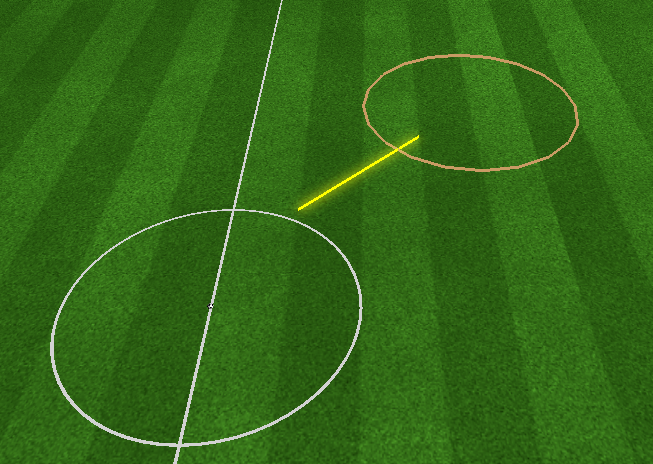
\includegraphics[scale=0.5]{CodeBeispielDraw} 
\end{center}
\caption{Ergebnis}
\end{figure}\\
